
% JuliaCon proceedings template
\documentclass{juliacon}
\setcounter{page}{1}

\begin{document}

% **************GENERATED FILE, DO NOT EDIT**************

\title{BlankLocalizationCore.jl: implementing blank localization in Julia}

\author[1, 2]{Tamás Cserteg}
\author[1]{András Kovács}
\author[1, 3]{József Váncza}
\affil[1]{EPIC Centre of Excellence, HUN-REN Institute for Computer Science and Control (SZTAKI), Budapest H-1111, Hungary}
\affil[2]{Doctoral School of Informatics, ELTE Eötvös Loránd University, Budapest H-1117, Hungary}
\affil[3]{Department of Manufacturing Science and Technology, Budapest University of Technology and Economics, Budapest H-1111, Hungary}

\keywords{Julia, Optimization, Machining, Blank localization}

\hypersetup{
pdftitle = {BlankLocalizationCore.jl: implementing blank localization in Julia},
pdfsubject = {JuliaCon 2022 Proceedings},
pdfauthor = {Tamás Cserteg, András Kovács, József Váncza},
pdfkeywords = {Julia, Optimization, Machining, Blank localization},
}


%TODO: ha kell hely, akkor Jóska BME-t törölhetjük

\maketitle

\begin{abstract}

Blank localization (also known as workpiece referencing) is an essential task in machining.
It aims to precisely establish the geometric relation of the machine tool (mill, lathe, etc.) and the workpiece.
We introduced the concept of multi-operation blank localization to address this task for drilling and milling scenarios in a semi-automated way,
%TODO: innentől a mondat második fele cut?
which allows positioning different machining features (e.g., different holes) separately in order to exploit the tolerances on the relative position of those features to compensate the small errors of the blank.
The method takes as input the measured rough geometry and the machining CNC code, and computes the best possible position of each feature considering machining allowances and tolerances by solving a convex quadratically constrained quadratic program (QCQP).
The versatility and extensibility of the Julia language helped the development of this algorithm, materializing in the \texttt{BlankLocalizationCore.jl} package.
Its flexibility and ease of use make it an excellent research tool that can be deployed in production as well.
\end{abstract}

\section{Introduction}
\label{sec:intro}
Cast parts may have small geometric variations from lot to lot that need to be addressed before machining by altering the CNC code.
Current practice is dominated by iterative adjustments by the human operator, which requires highly trained workers, takes a long time, and still, may produce scrap.
%TODO: kell egyáltalán ezeket hivatkozni?
Automated methods exist for complex free-form parts like wind turbines that place the entire blank as a single solid object \cite{ding:2021_CoarsefineOptimizationMethod}\cite{tan:2014_UnconstrainedApproachBlank}.
Multi-operation blank localization~\cite{cserteg:2023_Annals} however handles group of features independently providing greater flexibility than traditional approaches.
It focuses on drilling and milling which are among the most common machining operations, making it applicable to a wide range of products.
The abstract method and its implementation were developed in parallel, which required a language with support for easy prototyping and wide variety of tools.
Exactly for these reasons we chose the Julia language~\cite{bezanson2017julia}.

\section{Multi-operation blank localization}
\label{sec:algo}

The problem involves looking for the optimal position for each to-be-machined feature (short: machined feature) on the workpiece.
Based on the actual machining operations, these features are grouped into feature groups, for example, drilled holes on the same side of the part, whose drilling positions are defined relative to a common reference (the part zero).
Features within the same group move together, but different feature groups can move separately.
The machined features need to "enclose" the pre-cast features on the blank (called rough features) with a minimum machining allowance which ensures the required surface finish.
While doing so, the dimensional tolerances between some features need to be respected, as these describe functional properties (e.g. connections to mating parts).
Fig.~\ref{fig:hatfig} from \cite{cserteg:2023_Annals} shows an example of these features.

\begin{figure}[hbt]
	\centerline{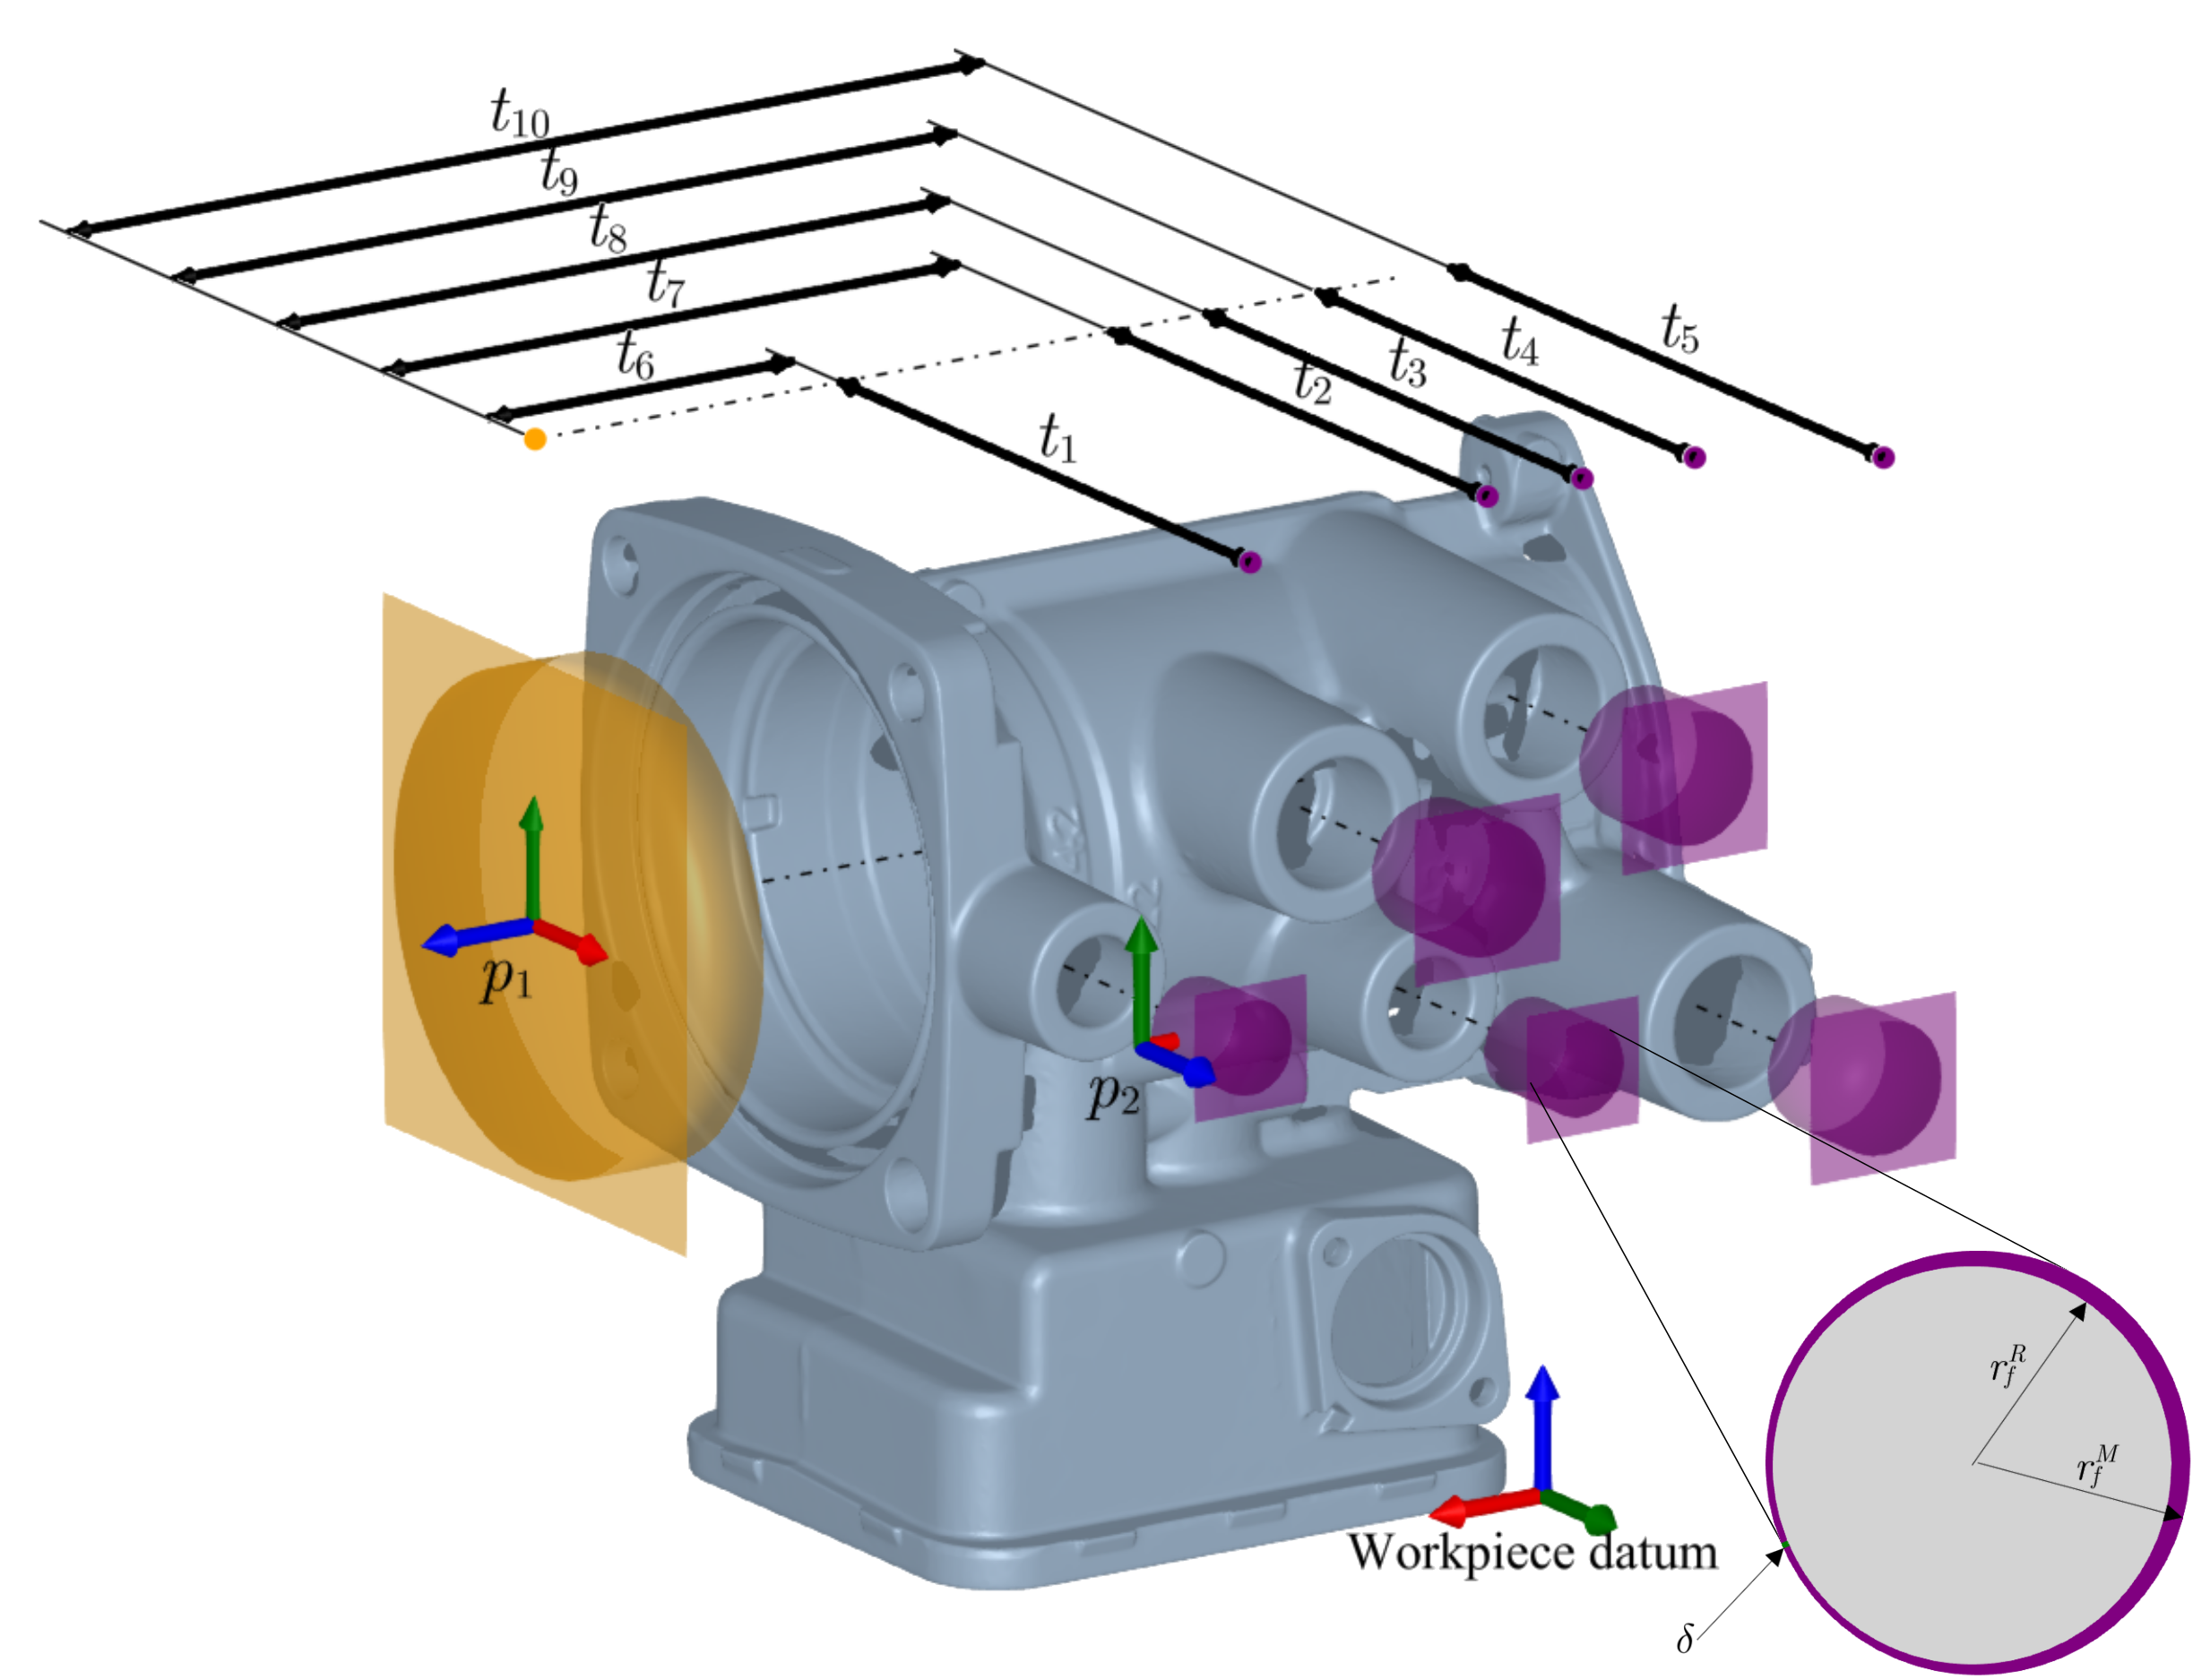
\includegraphics[width=0.95\columnwidth]{cirp-annals-2023-figure-2.png}}
	\caption{3D scanned rough features (in grey), two machined feature groups (orange and purple) with their part zeros, and tolerances connecting features \cite{cserteg:2023_Annals}.}
	%\caption{Measured part with two machined feature groups and tolerances between them. $r^M$ and $r^R$ denote the machined and rough radii of a feature, while $\delta$ the machining allowance \cite{cserteg:2023_Annals}.}
	\label{fig:hatfig}
\end{figure}

Following common machining practice the objective of the optimization program is to achieve as little tolerance deviation as possible, while ensuring that material is removed for proper surface finish.
The features are moved through their part zeros, which are the variables of the developed convex quadratically constrained quadratic program (convex QCQP).

A tolerance model was developed to replicate the tolerances used in design and machining process.
This model encodes the distance of machined-machined (or sometimes machined-rough) features as axis-aligned minimum and maximum distance.
These distances form constraints in the optimization program, while minimizing the deviation relative to their mean (central?) value across all tolerances is the objective function itself.

The allowance calculation requires the final part specification in the form of the machining CNC code as well as a representation of the rough geometries.
From these input data the rough-machined feature geometry pairs need to be extracted so that their machining allowance can be computed.
The geometric parameters are extracted so the constraint equations for the minimum machining allowance can be generated for the optimization program.

The optimization model itself and use-cases are described in \cite{cserteg:2023_CMS} and \cite{cserteg:2023_Annals}, while implementation details are given in the following section.

%These feature points can be a point of a plane or the center point of the end face of a cylinder for example.
%The former encodes the requirement that material needs to be removed to ensure proper surface finish and is described for a feature as the smallest thickness of removed material.
%A dimensional tolerance between two features is modeled as lower and upper bounds on the distance between the two features.
%As feature groups move together, only inter-group tolerances need to be considered.


%Briefly we can summarize the multi-operation blank localization as a method that aligns the machined and rough geometries with the required minimum overlap.
%It does it while making sure that features that are connected by dimensional tolerances are within the required distance range.

%Tolerance model is used
%Geometric computations
%Those two are bundled in a convex optimization problem.

%TODO: kihagyni a feature pontokat egy az egyben: Distance of freatures
%mi a feladat és milyen követelményeket támaszt az implementáció felé
% előbb feladatról beszélni és utána julia implementáció követeleményekről?
%todo: deklaratív megoldás
% feladat specifikáció: rough leírás, megmunkálandó leírás, toleranciák (alkatrészrajz, cnc kód)
% ebből a sokféle adatból készül a modell
%modellépítés: összes korlátot és célfv-t definiálni kell és annak az összes paraméterét ki kell számolni
% a geometriai számítűsok ahhoz kellenek, hogy kigeneráljuk a modell egyenleteit, amiknek önmagukban nincs jelentésük, mert csak egyenlőtlenségek.
%megoldás: darál a solver. Nem csinálunk semmit. - tök általános célú QCQP solver, aminek az eredményét valahogy implementálni kell
% kimenteni a part zerokat, és kiértékelni, hogy tolerancia ígyúgy, allownace ezaz meg vizualizáció

%todo az absztrakt modellépítést implementálja a julia implementáció sokkal részletesebben
% modellépítés és instancia generálás
% modellépítés, mint adatokkal való feltöltés <- ezt a julia csinálja
%The tolerance evaluation is part of the objective of the optimization model which means that the distance of these features needs to be often calculated.
%The distance of these features points, thus the evaluation of the tolerance depends on the position of these features which means that the tolerance values need to be evaluated while solving the optimization model.

%Evaluating the minimum machining allowance contributes to the constraints of the optimization program and depends on geometric calculations as well.
%The allowance calculation requires the position of the features as well as other geometric parameter (radii of cylinders for example).
%TODO: még egy mondat?


%While an appropriate solver is needed for this family of problems, the solver also needs to evaluate the above described tolerance model and geometric queries during solution.
%We detail this interaction in the next section, while the algorithm itself is described in \cite{cserteg:2023_CMS} and \cite{cserteg:2023_Annals}.

\section{Implementation in Julia}
\label{sec:approach}

During the development of the algorithm, we needed a software tool that supports the quick prototyping needs of research, while giving a solid foundation to validate the concept with our industry partner.
We needed a tool that:

\begin{itemize}
	\item Interfaces our model to the optimization solver and enables rapid prototyping.
	\item Supports a variety of geometrical representations, especially regarding the differences of drilling/milling operations and free-form/primitive geometry representation.
	\item Supports importing geometries from a variety of measurement tools (CMM, 3D scanner, measurement arm).
%	\item Supports easy extension of the geometries if required.
%	\item Supports extending 
%	\item Translates the tolerance model for the optimization solver.
	\item Supports easy debugging and helps analyzing and visualizing the results.
\end{itemize}

The heart of the implementation is the solver provided by the JuMP ecosystem~\cite{Lubin2023}.
With JuMP's excellent design, implementing the optimization model was as easy as repeating the mathematical model in Julia.
Other advantage of the JuMP ecosystem is that solvers can be easily swapped if needed.
For development, the FICO Xpress solver was used, but our industry partner could use the Ipopt or SCIP solvers without issue.

%TODO: azt kell elmagyarázni, hogy különböző geometria reprezentációk vannak különböző mérésekből
% de nekünk mindig ugyanaz az információ: a feature point kell
% és ezzel az interfésszel mindenféle mérőeszköz formátumát le tudjuk kezelni
% és van egy egységes interface a feautre pointok (geometriaia leírók, paraméterek?) lekérdezéséhez

To generate the optimization model we needed to store the 1. nc code 2. rough geometry 3. tolerances.
A common thing regarding the first two, that some kind of geometric representation is needed.
Representing the NC code can be done with plane and cylinder geometries for milling and drilling operations.
While the rough geometry poses greater challanges.
Different measurements instruments output different type of geometric data, for example a coordinate measurement arm (CMM) will provide primitive geometry definitions like disks and cylinders while a 3D scanner output point clouds or meshes (pongyolán csak free form).
Property of the optimization model is that it is built around "feature points" (consistently defined points of different geometries).
These two aspects required us to develop a type tree.
To cover our current needs (drilling and milling operations), planar and cylindrical geometries are defined.
The other property of geometries is if they are primitive or free form, which is covered by the holy trait pattern.
\texttt{IsPrimitve} or \texttt{IsFreeForm} traits can be applied to geometry types independently of their planar or cylindrical type.
Code block~\ref{lst:def-types} shows the core of the implementation of the type system.

\begin{lstlisting}[language = Julia, numbers=left, label={lst:def-types}, caption={Draft of the type system used by \texttt{BlankLocalizationCore.jl}.}]
# Supertype for localization geometries.
# "A": abbr. for Abstract
# "L": abbr. for Localization
abstract type ALocGeometry end
abstract type AHoleGeometry <: ALocGeometry end
abstract type APlaneGeometry <: ALocGeometry end

# Trait to describe the "style" of an ALocGeometry.
abstract type GeometryStyle end
struct IsPrimitive <: GeometryStyle end
struct IsFreeForm <: GeometryStyle end
\end{lstlisting}

The other part of the optimization generation interface is definition of the query functions that work on these types.
Free form geometries need to implement the \texttt{surfacepoints} and \texttt{filteredsurfacepoints} methods;
Primitive geometries need to have the \texttt{featurepoint} method and cylindrical features need the \texttt{featureradius} on top of that.
For visualization the \texttt{visualizationgeometry} function need to be defined whose output is passed to \texttt{Meshes.viz} function, so Meshes objects are needed.
A short example for such a definition is shown in code block~\ref{lst:example}.

The visulization interface is built around Meshes.jl, therefore the to-be-showed geometries must be from that package.
Using the Meshes ecosystem, we could produce publication quality images, like Fig.~\ref{fig:hatfig} from \cite{cserteg:2023_Annals}.

\begin{lstlisting}[language = Julia, numbers=left, label={lst:example}, caption={Defining a new type.}]
struct MyDisk <: AHoleGeometry
  p::Vector{Float64} # center point
  n::Vector{Float64} # surface normal
  d::Float64 # diameter
end
GeometryStyle(::Type{MyDisk}) = IsPrimitive()

featurepoint(::IsPrimitive, x::MyDisk) = x.p
featureradius(::IsPrimitive, x::MyDisk) = x.d/2

using Meshes

function visualizationgeometry(geom::MyDisk)
  plane = Plane(Point3(geom.p), Vec3(geom.n))
  return Disk(plane, geom.d/2)
end
\end{lstlisting}



The optimization program uses a feature point (or feature points for free form geometries) of features, that is used for computing the machining allowance and the dimensional tolerances.
A function interface is defined for querying these feature points of geometries, that is used to generate the optimization program.
Code block~\ref{lst:example} shows the definition of those functions as well.
The visulization interface is built around Meshes.jl, therefore the to-be-showed geometries must be from that package.
Using the Meshes ecosystem, we could produce publication quality images, like Fig.~\ref{fig:hatfig} from \cite{cserteg:2023_Annals}.


The optimization generation engine uses the functions defined by this interface to construct the optimization program.

As mentioned earlier, an important requirement was to handle the output formats of many different devices.
Every measurement instrument comes with its own processing software and export formats, not necessarily designed for interoperability.
As a result, we needed to write (or use) parsers for different text and tabular formats.

\section{Results and future work}
\label{sec:results}
%TODO
Future plans for the package and the method itself include an overhaul of the tolerance modeling scheme.
Currently, only dimensional tolerances are handled, but it should be discovered if more GD\&T tolerances can be incorporated into the model.
The current implementation supports only cylinders and planes, thus drilling and milling; it is a future research direction to extend the handled machining operations, e.g., to turning.

\section{Acknowledgments}
The research was supported by the European Union within the framework of the National Laboratory for Autonomous Systems (RRF-2.3.1-21-2022-00002) and the TKP2021-NKTA-01  NRDIO grant on "Research on cooperative production and logistics systems to support a competitive and sustainable economy".

% **************GENERATED FILE, DO NOT EDIT**************

\bibliographystyle{juliacon}
\bibliography{ref.bib}


\end{document}

% Inspired by the International Journal of Computer Applications template
